\section{Experiments} \label{sec:krd_experiments}
We implemented the above techniques in \krd, our system for \underline{Ru}le \underline{Di}scovery in \underline{K}nowledge Bases.
We carried out an extensive experimental evaluation of our approach and grouped the results in four main sub-categories: 
\begin{inparaenum}[\itshape(i)]
	\item demonstrating the quality of our output for positive and negative rules;
	\item comparing our method with the state-of-the-art systems;
	\item showing the applicability of rule discovery in Machine Learning algorithms with representative training data;
	\item testing the role of the parameters in the system. % settings and some KB properties.
\end{inparaenum}
%DO WE EVALUATE SAMPLING ON A DIFFERENT SECTION?

\myparagraph{Settings}
%We evaluated our approach over several popular KBs. 
%For each KB, 
%We downloaded the most up-to-date core facts and loaded them into our SPARQL query engine. We experimented with several SPARQL engines, 
%not relevant discussing sparql engines
%including \system{Jena ARQ}\footnote{\url{https://jena.apache.org/documentation/query/}}, \system{OWLIM %Lite}\footnote{\url{https://confluence.ontotext.com/display/OWLIMv54/OWLIM-Lite+Installation}}, and %\system{RDF-3x}\footnote{\url{https://code.google.com/archive/p/rdf3x/}}. We also implemented a na\"ive %relational database solution with \system{PostgreSQL}. 
%and eventually we opted for \system{OpenLink Virtuoso},
%\footnote{\url{http://virtuoso.openlinksw.com/}}
%as it was the fastest among all the solutions. 
%\system{Virtuoso} took on average 20 minutes to load a medium size KB (i.e., 10 GB) into its store, and %around 100 milliseconds to execute a single hop query. 
We ran experiments over the latest core facts derived from several KBs. All experiments were run on a desktop with a quad-core i5 CPU at 2.80GHz and 16GB RAM. We used \system{OpenLink Virtuoso}, optimized for 8GB RAM, with its SPARQL query endpoint on the same machine.

%In the following, 
Parameters $\alpha$ and $\beta$ of Equation~\ref{eq:weight_fun} were set to  $\alpha=0.3$ and $\beta=0.7$ for positive rules, and to $\alpha=0.4$ and $\beta=0.6$ for negative rules. 
%We also use a $maxPathLen$ parameter indicating the maximum number of atoms in each of the rules to be discovered that is set to $3$. 
We set the maximum number of atoms 
admissible in the body of a rule ($maxPathLen$) to $3$.
We analyze the role of these parameters in Section~\ref{sec:krd_int_evaluation}. 
\begin{comment}
Our method needs the two input parameters $\alpha$ and $\beta$ of Equation~\ref{eq:weight_fun}. 
We set $\alpha=0.3$ and $\beta=0.7$ for positive rules, while $\alpha=0.4$ and $\beta=0.6$ for negative rules. We empirically justify this choice in Section~\ref{sec:krd_int_evaluation}.
%$\alpha$ measures the importance of the coverage over the generation set, while $\beta$ measures the coverage over the validation set. In other words, a high $\alpha$ privileges recall over precision, while a high $\beta$ gives more importance to precision. We can afford a high $\alpha$ and a low $\beta$ when the input KB is accurate and complete. We will show that KBs contain many errors and missing information, therefore we set $\alpha = 0.3$ and $\beta = 0.7$. Increasing $\alpha$ and decreasing $\beta$ means a higher number of output rules with a lower accuracy. 
We also set the $maxPathLen$ parameter to $3$. This number represents the maximum number of atoms that we can have in the body of a rule. We will outline in Section~\ref{sec:krd_int_evaluation} that increasing this parameter does not bring any benefits, as rules with a body longer than $3$ atoms start to be very complicated and not insightful.
\end{comment}

\myparagraph{Evaluation Metrics}
We evaluated the effectiveness of \krd in discovering both positive and negative rules. The set of predicates for evaluation were chosen separately in the case of positive and negative rules from each KB.
For every KB, we first ordered predicates according to descending popularity (i.e., number of triples having that predicate). We then picked the top $3$ predicates for which we knew there existed at least one meaningful rule, and other $2$ top predicates for which we did not know whether some meaningful rules existed or not. 
%: we picked $5$ popular predicates occurring in a majority of triples out of which the top $3$ are known to have at least one meaningful rule, while there is no prior knowledge about the rules for the next 2 predicates. 

The evaluation of the discovered rules 
%discovered by \krd and the baseline algorithms we compare against 
%was done for both positive and negative rules 
has been done according to the state of the art for rule quality evaluation~\cite{galarraga2015fast}. If a rule was clearly semantically correct, we marked all its results over triples as true. If a rule correctness was unknown, we randomly sampled 30 triples either among the new facts (for positive rules) or among the errors (for negative rules), 
%new predictions likely to be violating rule head 
and manually checked them. % against the Web. 
The \emph{precision} of a rule is then computed as the ratio of correct assertions out of all assertions. 
%The subtle difference is that the sample set of tentatively violating predictions to be evaluated are generated differently for positive and negative rules. As an example, for the positive rule $\atom{spouse}{a}{v0} \wedge \atom{child}{v0}{b} \Rightarrow \atom{child}{a}{b}$, we retrieve all those pairs  $(a,b)$ such that $b$ is the child of $v0$ and $v0$ is the spouse of $a$ but $b$ is not the child of $a$. In the case of the negative rule, $\atom{child}{a}{b} \Rightarrow \neg \atom{spouse}{a}{b}$, we retrieve all those pairs $(a,b)$ such that $b$ is \texttt{child} of $a$ and $a$ is \texttt{spouse} with $b$.
\begin{comment}
\krd discovers rules for a given target predicate. For each KB, we chose $5$ representative predicates as follows: we first ordered predicates according to descending popularity (i.e., number of triples having that predicate), and then we picked the top $3$ predicates for which we knew there existed at least one meaningful rule, and other $2$ top predicates for which we did not know whether some meaningful rules existed or not. We repeated the procedure for each input KB, and for both positive and negative rules. Despite working with one predicate at a time, \krd can also discover rules for the entire KB by enumerating all the predicates in the KB, and discovering rules for each of them. We will show in Section~\ref{sec:krd_comparative} how this can be achieved.

Positive rules are very useful to enrich the KB by discovering new facts. 
%Since we are generating new data, we cannot evaluate the output over the existing data. 
Inspired by~\cite{galarraga2015fast}, we proceed as follows: we run the algorithm over the KB, and for each output rule we generate all new predictions that are not already in the KB (we execute the body of the rule against the KB and remove all those pairs that are already connected by the target predicate in the KB). 
%As an example, for the rule $\atom{spouse}{b}{a} \Rightarrow \atom{spouse}{a}{b}$, we retrieve all pairs %$(b,a)$ such that $b$ is \texttt{spouse} with $a$ but $a$ is not \texttt{spouse} with $b$ in the KB. 
If a rule is universally correct 
%(like the previous example)
, we mark all its new predictions as true. If a rule is unknown, we randomly sampled 30 new predictions and manually checked them against the Web. The \emph{precision} of a rule is then computed as the ratio of true predictions out of true and false predictions.

Negative rules are slightly more complicated to evaluate. In fact, despite KBs being usually incomplete, a large percentage of the data not stated in a KB is false. 
%-- a very small fraction of the cartesian product of all the people in a KB will be actually married.
Therefore negative rules will always discover many correct negative facts. However, negative rules are a great means to discover errors in the KB, and we leverage this aspect to evaluate them. For each discovered rule, we retrieve from the KB the pairs of entities for which the body of the rule can be instantiated over the KB and that are also connected by the target predicate. As an example, for the rule $\atom{child}{a}{b} \Rightarrow \neg \atom{spouse}{a}{b}$, we retrieve all those pairs $(a,b)$ such that $b$ is \texttt{child} of $a$ and $a$ is \texttt{spouse} with $b$. We call these generated pairs of entities \emph{potential errors}. Similar to positive rules, whenever a rule is universally correct we mark all its potential errors as true, whereas if the rule is unknown we manually check 30 sampled potential errors. The final precision of a rule is computed as actual errors divided by potential errors.


%The following can be skipped
%Furthermore, a potential error is evaluated as actual error whenever a single atom in the rule is incorrect, no matter if the atom is in the body or the head of the rule. For the negative rule $\atom{child}{a}{b} \Rightarrow \neg \atom{spouse}{a}{b}$, a specific instantiation $(a,b)$ is an actual error if either $b$ is not an actual \texttt{child} of $a$, or $b$ is not an actual \texttt{spouse} of $a$. As we will explain further below, negative rules cannot point exactly where the error is, but they give a hint that something is wrong and needs to be further inspected.
\end{comment}

Full test results, including KBs, induced rules, annotated examples and rules are available at \url{http://bit.ly/2csROsc}.


%\vspace{-1ex}
{\small
\begin{table}[thb]
	\centering
	\caption{Dataset characteristics.}
	\label{tab:krdDatasetDescr}
	\begin{small}
		\begin{tabular}
			{|>{\centering}m{1.2cm}|>{\centering}m{1.1cm}|>{\centering}m{1.15cm}|c|>{\centering}m{1.5cm}|}
			\hline
			\hline
			{\it KB}&{\it Version}&{\it Size}&{\it  \#Triples}&{\it \#Predicates} \tabularnewline
			\hline
			\dbpedia & 3.7 & 10.056GB & 68,364,605 & 1,424 \tabularnewline
			\yago & 3.0.2 & 7.82GB & 88,360,244 & 74 \tabularnewline
			\wikidata & 20160229 & 12.32GB & 272,129,814 & 4,108 \tabularnewline
			\hline
		\end{tabular}
	\end{small}
\end{table}
}

\vspace{-1ex}
\subsection{Quality of Rule Discovery in \krd} \label{sec:gen_evaluation}
\vspace{-1ex}
The first set of experiments aimed at evaluating the accuracy of discovered rules over three popular KBs: \dbpedia~\cite{bizer2009dbpedia}, \yago~\cite{suchanek2007yago}, and \wikidata~\cite{vrandevcic2014wikidata}. 
%For each KB we downloaded the most recent version and selected core facts, facts about people, geolocations and transitive \texttt{rdf:type} facts. \wikidata provides the entire dump alone; therefore we just eliminated from it all the non-English literal values. 
Table~\ref{tab:krdDatasetDescr} shows the characteristics of the KBs.

%As the figure shows, 
The size of the KB is important as loading the entire KB in memory is not feasible unless we either have HW with large amount of memory~\cite{Chen:2016,DBLP:conf/sigmod/FaridRIHC16}, or we shrink the KB by eliminating all the literals~\cite{galarraga2015fast}. In our approach, only a small portion of the KB is loaded in memory, thus we can afford to (i) discover rules with commodity HW resources, (ii) retain the literals, which are crucial for the value comparison in our rules. While \krd mines rules for a given target predicate at a time, it discovers rules over the entire KB given its set of predicates. This is further elaborated in Section~\ref{sec:krd_comparative}.

\begin{table}[ht]
%\vspace{-2ex}
	\centering
	\caption{\krd Positive Rule Accuracy.}
	\label{tab:pos_rules_acc}
	\begin{small}
	\begin{tabular}{|c|c|c|c|c|}
		\hline
		\hline
		{\it KB}&{\it Avg. Run Time}&{\it Avg. Precision}&{\it \# Annotations} \tabularnewline
		\hline
		\dbpedia & 34min, 56sec & \textbf{63.99}\% & 139\tabularnewline
		\yago &  59min, 25sec & \textbf{62.86}\% & 150\tabularnewline
		\wikidata &  2h, 21min, 34sec & \textbf{73.33}\% & 180\tabularnewline
		\hline
	\end{tabular}
	\end{small}
\end{table}
\vspace{-1ex}


\myparagraph{Positive Rules \krd} 
We first evaluate the precision for the positive rules on the top 5 predicates for each KBs. 
The number of new induced facts varies significantly from rule to rule.
% -- a rule with literals comparison produces a very high number of facts. In order 
To avoid the overall precision to be dominated by such rules, we first compute the precision for each rule as explained above, and then average values over all induced rules.
 Table~\ref{tab:pos_rules_acc} reports precision values, along with predicates average running time.
 Column \emph{\# Annotations}  reports the size of the sample of manually annotated triples.



Results show that the more accurate is the KB, the better is the quality of the induced rules. \wikidata contains very few errors, since it is manually curated, while
%and every triple is manually checked by different individuals before being inserted
 \dbpedia and \yago are automatically generated by extracting information from the Web, hence their quality is significantly lower. 
\begin{comment}
Discovering perfect positive rules is a hard task, mostly because there is no guarantee of the existence of valid negative examples. A striking example in this direction is one of the rule induced for \texttt{founder} in \dbpedia. Our approach discovers that if a person is born in the same place where a company is founded, then the person is the founder. The rule is obviously wrong
%, as there are many people who are born in the same place of a company and have not founded the company
. However this rule has a very high coverage over the generation set (many companies' founders founded their company in their birth place), and a very low coverage over the validation set -- among the cartesian product of all the people and companies, a very small fraction includes people and companies born and founded in the same place. Despite such hard cases, our approach is always capable of producing correct rules for those predicates for which we knew there existed some valid rules. 
\end{comment}
Some predicates, such as \texttt{academicAdvisor}, \texttt{child}, and \texttt{spouse}, have a precision above $95\%$ in all KBs, but average precision values are brought down by few predicates, such as \texttt{founder}, where meaningful positive rules probably do not exist at all. In other terms, when a rule exists, the system was able to find, but it was not able to recognize cases where no positive rules exist (indeed it is not possible to derive a founder from the information on persons and company in the KBs). 

The running time is influenced by the size of the KB with the number of triples and the number of predicates. %\krd is slower in \wikidata, which is the biggest KB.
 The more predicates we have in the KB, the more alternative paths we test while traversing the graph.
% thus resulting in a bigger search space. 
Another relevant aspect is the target predicate involved. Some entities have a huge number of outgoing and incoming edges, entity ``\textit{United States}'' in \wikidata has more than $600$K. When the generation set includes such entities, the navigation of the graph is slower as we traverse a large number of edges. 
%This is what happens in \yago, where the most popular predicates are \texttt{isLeaderOf} and \texttt{exports}. 
Parameter $maxPathLen$  also impacts the running time. The longer the rule, the bigger is the search space, as we discuss in Section~\ref{sec:krd_int_evaluation}. 
%We will show in the next Section how we can be much faster if we set to 2 atoms the maximum length of the rule. In the next chapter we will discuss some future directions to significantly cut down the running time based on the above observations.


%\vspace{1ex}
\begin{table}[htb]
	\centering
	\caption{\krd Negative Rule Accuracy.}
	\label{tab:neg_rules_acc}
	\begin{small}
	\begin{tabular}{|c|c|c|c|}
		\hline
		\hline
		{\it KB}&{\it Avg. Run Time}&{\it \# Pot. Errors} & {\it Precision} \tabularnewline
		\hline
		\dbpedia & 19min, 40sec& 499 (84) & \textbf{92.38}\%\tabularnewline
		\yago & 10min, 40sec & 2,237 (90) & \textbf{90.61}\%\tabularnewline
		\wikidata & 1h, 5min, 38sec & 1,776 (105)& \textbf{73.99}\%\tabularnewline
		\hline
	\end{tabular}
	\end{small}
\end{table}

\myparagraph{Negative Rules \krd} 
%Negative rules are very useful to discover inconsistencies in the KB. 
We evaluated negative rules as the percentage of correct errors discovered for the top 5 predicates in each KB. Table~\ref{tab:neg_rules_acc} shows, for each KB, the total number of potential erroneous triples discovered with the rules, whereas the precision is computed as the percentage of actual errors among potential errors. Numbers in brackets show the sample of unknown triples manually annotated.

Negative rules have better accuracy than positive ones. 
This is due to the fact that negative rules exist more often then positive rules.
% completeness of the validation set: for negative rules the validation set is the universe of all possible counter examples stated in the KB, whereas for positive rules the validation set is a small fraction of it. %Therefore negative rules are usually better validated than positive ones. 
%As expected, for the manually curated \wikidata, the precision of the rules is higher, and the absolute number of errors identified is lower because it does not contain as many errors as \dbpedia and \yago.
%For example, we identify the same rule that two people with same gender cannot be married both in \yago and \wikidata. Such a rule has a 94\% precision in \yago, while the accuracy in \wikidata is 57\%.
 \yago has the highest number of errors; for example, there are $9,057$ cases in the online \yago where a child is born before the parent. 
%We cannot point exactly where the error is -- there could be an error in one of the birth dates or an error in the parent relation -- but we can affirm that at least one of these values is wrong and send them to human evaluators to spot the inconsistency.
%
Differently from positive rules, literals play a key role in negative rules. In fact, several correct negative rules rely on temporal aspects in which something cannot happen before/after something else. Temporal information are usually expressed through dates, years, or other primitive types that are represented as literal values in KBs.

Discovering negative rules is faster than discovering positive rules
%.This is due to the time spent executing 
because of the different nature of the examples covered by validation queries. 
Whenever we identify a candidate rule, we execute the body of the rule against the KB with a SPARQL query to compute its coverage over the validation set. 
These queries are faster for negative rules since the validation set is simply all the entities directly connected by the target predicate, whereas in the positive case the validation set corresponds to counter examples that do not have this property and are more expensive to evaluate for SPARQL engines.
%, as discussed in Section~\ref{sec:ex_generation}.

%DO NOT SHOW RULES EXAMPLES
%Table~\ref{tab:neg_rules_acc} shows some interesting cases, for both correct and incorrect rules.
%The example rules show the full power of our language, including literals, smart literals comparisons, entities inequalities and constants. As previously mentioned, the extension including literals comparisons and entities inequalities gives a significant boost in accuracy for negative rules, while it is rarely used in discovery positive rules. The full set of discovered rules can be inspected online (TODO: footnote online appendix).
%
%\begin{table}[htb]
%	\centering
%	\label{tab:krd_rules_example}
%	\begin{small}
%		\begin{tabular}{>{\centering}m{10cm}|c|c}
%			{\it Rule}&{\it KB}&{\it Precision} \tabularnewline
%			\hline
%			$\atom{notableWork}{b}{a} \Rightarrow \atom{creator}{a}{b}$ & \wikidata & \textbf{100}\% \tabularnewline
%			$\atom{nationality}{a}{v_0} \wedge \atom{nationality}{b}{v_0} \wedge \atom{notableStudent}{b}{a} \Rightarrow \atom{academicAdvisor}{a}{b} $ & \dbpedia & \textbf{100}\% \tabularnewline
%			$\atom{hasChild}{v_0}{b} \wedge \atom{isMarriedTo}{a}{v_0} \Rightarrow \atom{hasChild}{a}{b}$ & \yago & 50\% \tabularnewline
%			$\atom{activeYearsEndDate}{a}{v_0} \wedge \atom{activeYearsStartDate}{b}{v_0} \Rightarrow \atom{successor}{a}{b}$ & \dbpedia & 0\% 
%			\tabularnewline 
%			$\atom{inception}{a}{v_0} \wedge \atom{dateOfBirth}{b}{v_1} \wedge v_1 > v_0 \Rightarrow \neg \atom{founder}{a}{b} $  & \wikidata & \textbf{100}\% 
%			\tabularnewline 
%			$\atom{country}{a}{England} \wedge \atom{country}{b}{United\_Kingdom} \wedge England \neq United\_Kingdom \Rightarrow \neg \atom{county}{a}{b}$ & \dbpedia & \textbf{100}\% \tabularnewline
%			$\atom{actedIn}{a}{b} \Rightarrow \neg \atom{wroteMusicFor}{a}{b}$ & \yago & 40\% \tabularnewline
%			$\atom{birthYear}{a}{v_0} \wedge \atom{birthDate}{b}{v_1} \wedge v_0 < v_1 \Rightarrow \neg \atom{academicAdvisor}{a}{b} $  & \dbpedia & 28.6\% 
%		\end{tabular}
%	\end{small}
%	\caption{Interesting Output Rules.}
%\end{table}

\vspace{-1ex}
\subsection{Comparative Evaluation} \label{sec:krd_comparative}
\vspace{-1ex}
We compared our methods against \amie~\cite{galarraga2015fast}, the state-of-the-art positive rule discovery system for KBs.
%
\amie loads the entire KB into memory and discovers positive rules for every predicate. % in the KB. 
%\amie lists all the predicates in the KB and inserts each of them as head of the rule. Once the head is filled, the system tries to expand the rule by pivoting on one of the variables of the current predicate and looks for predicates sharing the same variable with high coverage in the KB. 
%The coverage of a rule is penalized with the partial closed world assumption, where the set of negative examples for a given pair $(x,y)$ and a target predicate $p$ is all those pairs where $x$ is connected through $p$ to an entity different from $y$. 
%Differently from us, 
It then outputs all possible rules that exceed a given threshold and ranks them according to a coverage function.

\begin{table}[htb]
%\vspace{-3ex}
	\centering
	\caption{\amie Dataset characteristics.}
	\label{tab:AmieDatasetDescr}
	\begin{small}
		\begin{tabular}{|c|c|c|c|c|c|}
			\hline
			\hline
			{\it KB}&{\it Size}&{\it  \#Triples}&{\it \#Predicates}&{\it \#}\texttt{rdf:type}\tabularnewline
			\hline
			\dbpedia & 551M & 7M & 10,342 & 22.2M \tabularnewline
			\yago & 48M & 948.3K & 38 & 77.9M  \tabularnewline
			\hline
		\end{tabular}
	\end{small}
\end{table}

Given its in-memory implementation, \amie went out of memory for the KBs of Table~\ref{tab:krdDatasetDescr} on our machine. Thus, we used the modified versions of \yago and \dbpedia from the \amie paper~\cite{galarraga2015fast}, which are devoid of literals and \texttt{rdf:type} facts.
%~\footnote{\url{www.mpi-inf.mpg.de/departments/databases-and-information-systems/research/yago-naga/amie/}}
%These versions consist of the core facts of the KB, without literals and \texttt{rdf:type} facts. Table~\ref{tab:AmieDatasetDescr} summarizes the characteristics of these datasets.
%
Removing literals and \texttt{rdf:type} triples drastically reduce the size of the KB. Since our approach needs type information (for the generation of $G$ and $V$ and for the discovery of inequality atoms), we run \amie on its original dataset, while for our algorithm we used the \amie dataset plus \texttt{rdf:type} triples. Last column of Table~\ref{tab:AmieDatasetDescr} reports the number of triples added to the original \amie dataset.

\myparagraph{Positive Rules Comparison} We first compared against \amie on its natural setting: positive rule discovery. \amie takes as input an entire KB, and discovers rules for every predicate in the KB. We adapted \krd to this setting as follows: we first list all the predicates in the KB, and for each predicate that connects a \emph{subject} to an \emph{object}. We then computed %the most common type 
for both subject and object %. The most common type is 
the most popular \texttt{rdf:type} that is not super class of any other most popular type. We finally ran our approach sequentially on every predicate, with $maxPathLen=2$ (\amie default setting).

%After computing type domain and co-domain for each predicate, we run our approach sequentially on every predicate. Furthermore we set the $maxPathLen$ parameter to 2, since this is the default setting for \amie.

\begin{figure}[htb]
	\centering
	\vspace{1ex}
	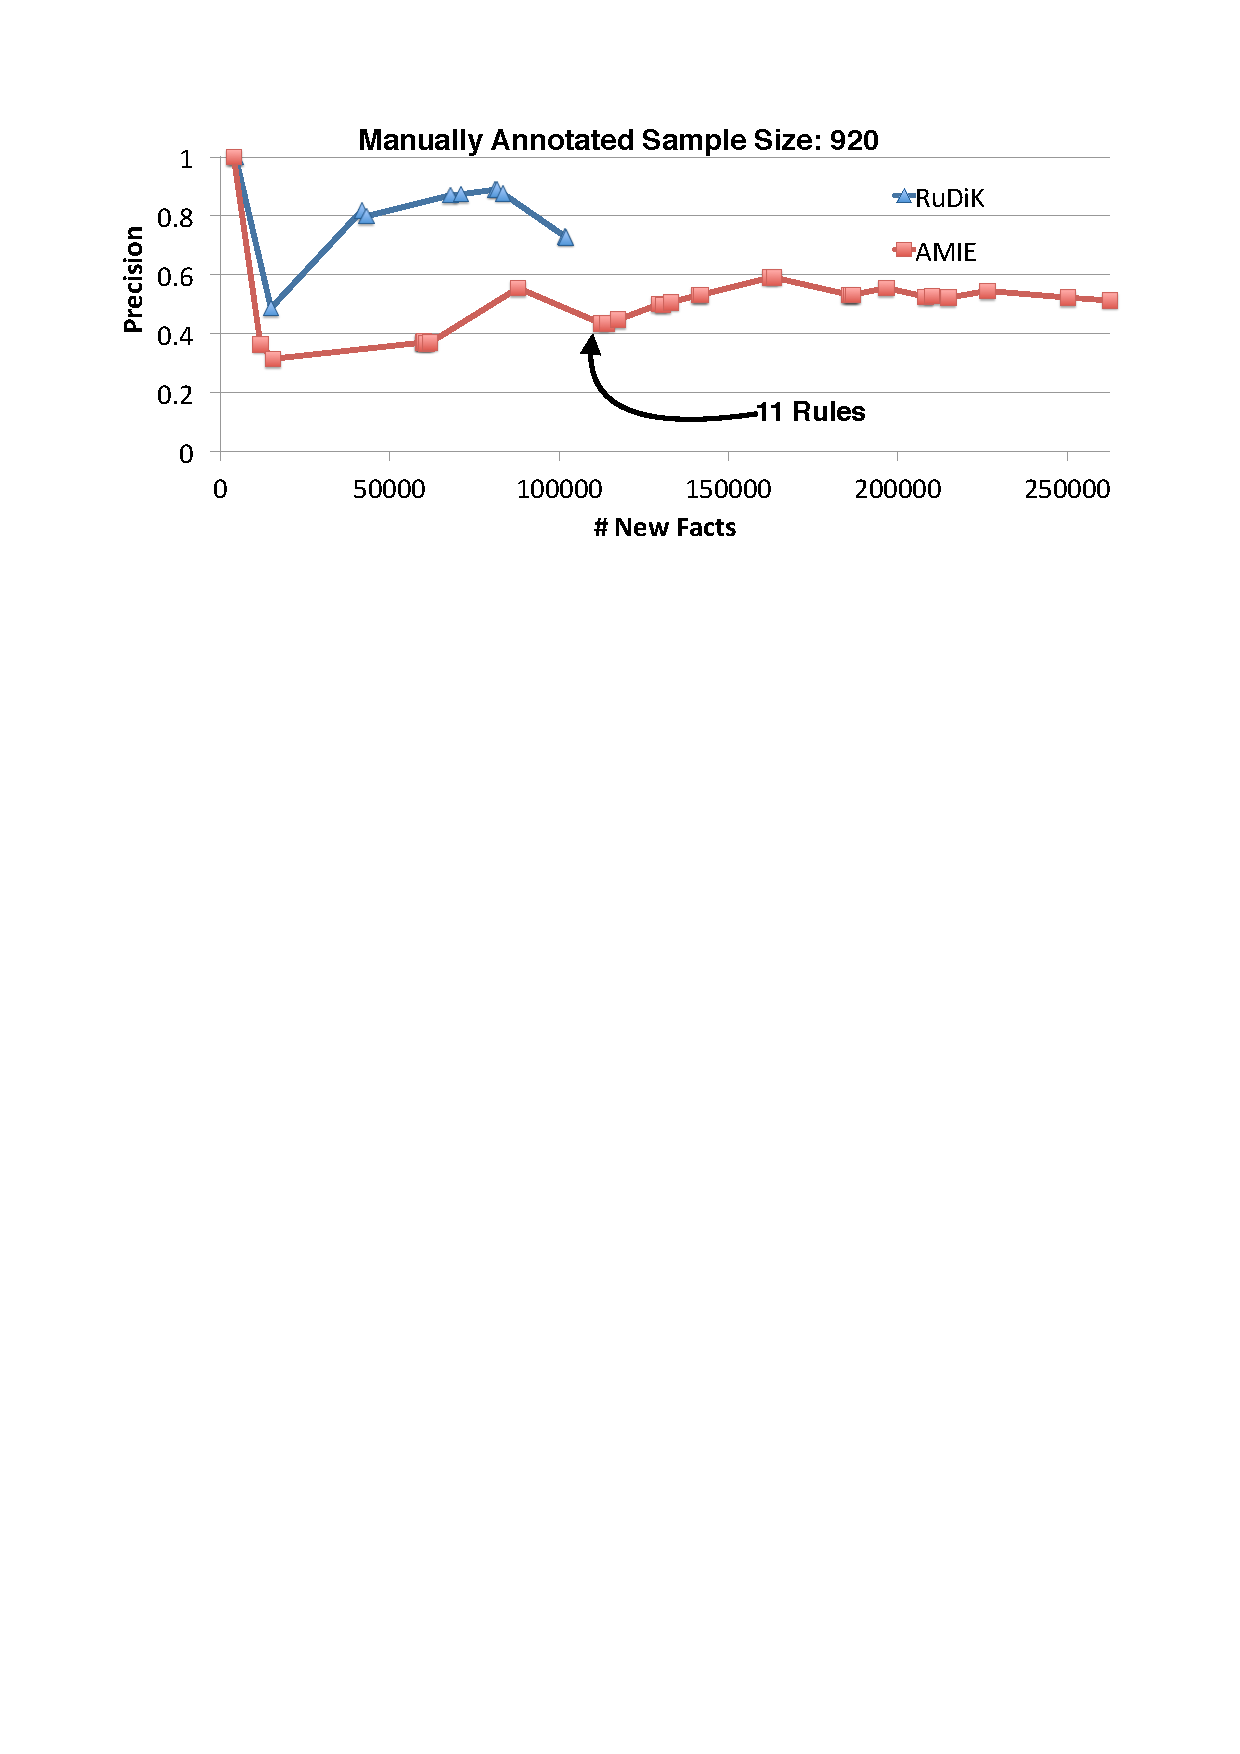
\includegraphics[width=.9\columnwidth]{include/figure/vsAmieYago.pdf}
	\vspace{-2ex}
	\caption{Accuracy for new facts identified by executing rules according to descending score on  \yago (no literals).}
	\label{fig:vs_amie_yago}
\end{figure}


\amie discovers 
%a huge amount of rules 
%along with their scores 
75 output rules in \yago, and 6090 in \dbpedia. We followed their experimental setting and picked the first 30 best rules according to their score. We then picked the rules produced by our approach on the same head predicate of the 30 best rules in the output of \amie. 
%I DON T UNDERSTAND LAST SENTENCE

\begin{figure}[ht]
	\centering
	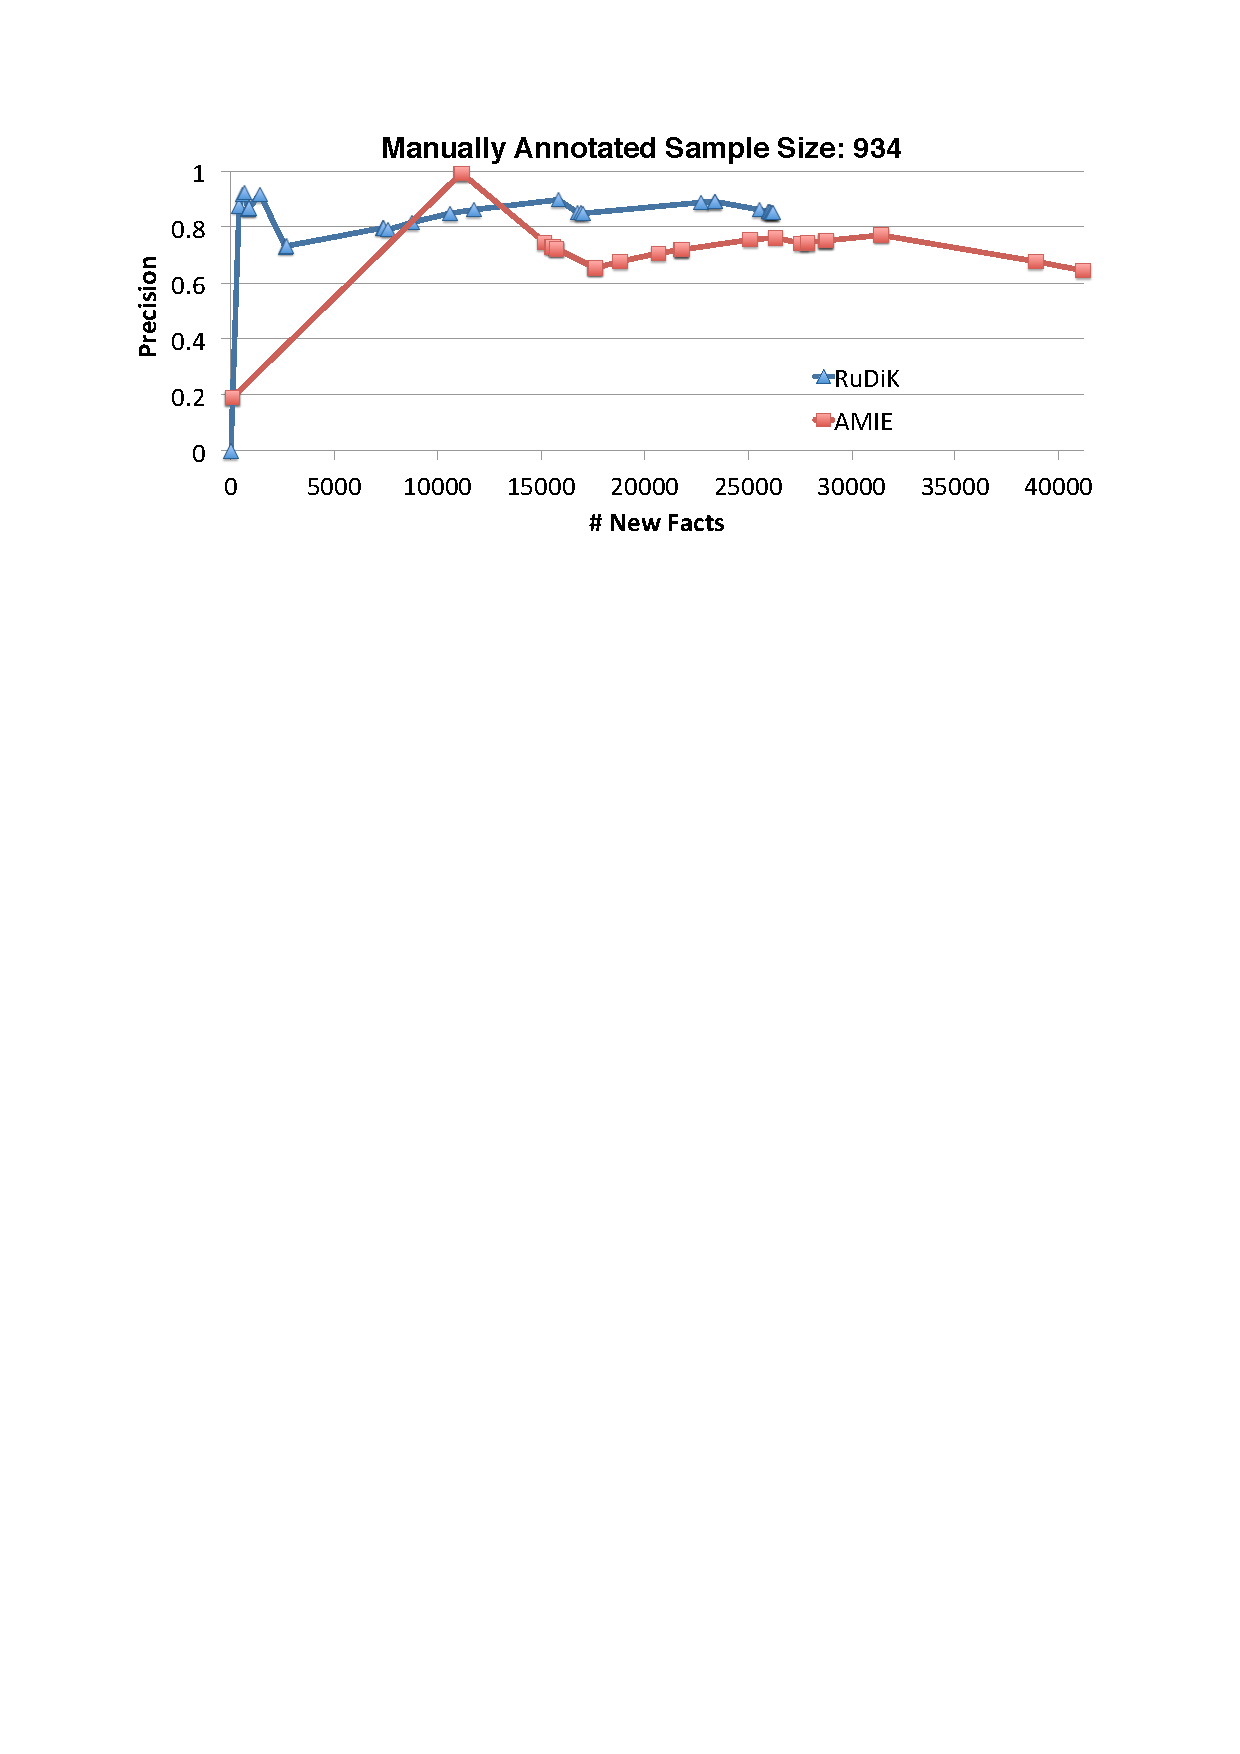
\includegraphics[width=.9\columnwidth]{include/figure/vsAmieDBPedia.pdf}
	\vspace{-2ex}
	\caption{Accuracy for errors identified by executing rules according to descending score on \dbpedia (no literals).}
	\label{fig:vs_amie_dbpedia}
\end{figure}

For this evaluation, we plot the total cumulative number of new unique predictions (x-axis) versus the aggregated precision (y-axis) when incrementally including in the solution the rules according to their descending score. Figures~\ref{fig:vs_amie_yago} and \ref{fig:vs_amie_dbpedia} report the results
on \yago and \dbpedia, respectively. 
Rules from \amie produce more predictions, but with a significant lower accuracy in both KBs. This is because, many good rules are preceded by meaningless ones in the ranking, and it is not clear how to set a proper $k$ to get the best top $k$ rules. 
In \krd, instead of the conventional ranking mechanism, we use a scoring function that discovers only inherently meaningful rules with enough support. 
%This approach is beneficial for the discovery, as shown  by the high precision we obtain %with a concise rule set 
%in both \yago and \dbpedia.
%
%\krd does not rely on a threshold and its algorithm identifies some of the cases when meaningful rules do not exist. % and it outputs a rule only when it has a strong confidence.
%is more conservative and produces much less rules than \amie. We noticed that for every predicate \amie always discovers more than one rule, while there are several predicates where the output of our algorithm is empty since none of the plausible rules has enough support. 
As a consequence, \krd outputs just 11 rules for 8 target predicates on the entire \yago -- for the remaining predicates \krd does not find any rule with enough support. If we limit the output of \amie to the best 11 rules in \yago (same output as our approach), its final accuracy is still 29\% below our approach, with just 10K more predictions.
%The only point where \amie outperforms our approach is upon \dbpedia when we consider the top $3$ rules: the third rule discovered by \amie is indeed a universally true rule that produces more than 11K correct predictions.
%NOT ESSENTIAL
%The precision of each rule is computed as described above with a minor modification: whenever a rule is unknown with its new predictions, we first check the existence of the new induced facts in a newer version of the KB. This is possible because the \amie dataset does not contain the most up to date versions. If a new fact does not appear neither in a newer version nor on the Web, it is evaluated as false.




%The $n$-th point from the left represents the total number of predictions and the total precision of these predictions, computed over the first $n$ rules (sorted according to \amie's score). 
%\amie produces many more predictions (262K vs 102K), but with a significant lower accuracy contrary to \krd which maintains a precision above 85\% before the last rule, with more than 80K predictions. This is due to the high number of rules in output of \amie, but also to the way these rules are ranked.

%NOT ESSENTIAL
%Moreover, our approach can also simulate \amie if we are more interested in recall. By modifying the $\alpha$ and $\beta$ parameters, we can obtain a higher number of predictions in output, at the expense of accuracy. 



%Figure~\ref{fig:vs_amie_dbpedia} shows the same evaluation on \dbpedia. \dbpedia has a richer set of relations, therefore also \krd is capable of producing 30 rules in output. Despite the same number of rules, once again our approach leads to a lower number of predictions (26K vs 41K) with a significant higher accuracy (85\% vs 74\%). The only point where \amie outperforms our approach is when we consider the top $3$ rules: the third rule discovered by \amie is indeed a universally true rule that produces more than 11K correct predictions.

\myparagraph{Negative Rules Comparison}
%We used \amie also to discover negative rules. 
\amie is not designed to discover negative rules, and can mine rules only for predicates explicitly stated in the KB. To use it as a baseline, we created a set of negative examples as explained in Section~\ref{sec:ex_generation} for each predicate in the top-5. To let \amie mine this information, for each negative example we added a new fact to the KB by connecting the two entities with the \emph{negation} of the predicate. 
For example, we added a \texttt{notSpouse} predicate connecting each pair of people who are not married according to our generation technique. We then run \amie on these new predicates. 
%The evaluation of negative rules is then carried out as explained before: we generate potential errors in the KB, and we manually evaluated the precision of such errors. 

\begin{table}[htb]
%\vspace{-3ex}
	\centering
	\caption{Negative Rules vs \amie.}
	\label{tab:vs_amie_neg}
	\begin{small}
		\begin{tabular}{c|c|c|c|c|}
			\cline{2-5}
			& \multicolumn{2}{c|}{{\amie}} & \multicolumn{2}{c|}{{\krd} (no literals)} \tabularnewline
			\hline
			\multicolumn{1}{ |c| }{\it KB}&{\it \# Errors} & {\it Precision} &{\it \# Errors} & {\it Precision} \tabularnewline
			\hline
			\multicolumn{1}{ |c| }{\dbpedia} & 457 (157) & 38.85\% & 148 (73) & \textbf{57.76}\%\tabularnewline
			\multicolumn{1}{ |c| }{\yago} & 633 (100) & 48.81\% & 550 (35) & \textbf{68.73}\%\tabularnewline
			\hline
		\end{tabular}
	\end{small}
\end{table}


Table~\ref{tab:vs_amie_neg} shows that \krd outperforms \amie in both cases with a precision gain of almost 20\%. The drop in quality for \krd w.r.t. the ones showed in Section~\ref{sec:gen_evaluation} is because we are using %the \amie modified 
KBs without literals.
Numbers in brackets show the number of triples manually annotated. 
% This is because for the negation of a predicate, we use the actual predicate as counter examples. \amie instead is not aware that the actual predicate provides counter examples for the negation of it, hence it is much less precise. In fact the output of \amie consists in a high number of rules for each predicate (often more than 30), and in many cases \amie produces same rules for both positive and negative scenarios. 
%As an example, \amie outputs that if a country $a$ exports a good $b$, then $a$ imports $b$ and $a$ does not import $b$. 

%NOT ESSENTIAL
%Despite clearly outperforming \amie, numbers look significantly lower that the ones showed in Section~\ref{sec:gen_evaluation}. This is because we are using the \amie modified KBs which do not contain literals. As explained earlier, literals play a vital role when discovering negative rules, both in terms of total errors discovered and in terms of precision. Excluding literals is a big disadvantage, and we will emphasise this aspect in detail in Section~\ref{sec:krd_int_evaluation}. (TO DO: check if the internal evaluation actually exists)

\myparagraph{Running Time}
%We report the running time of \amie compared to our approach. 
Running times for \amie are different from~\cite{galarraga2015fast}, where it was run on a 48GB RAM server. On our machine, \amie could finish the computation  on \yago 2, while for other KBs it got stuck after some time. For these cases, we stopped the computation if there were no changes in the output for more than 2 hours.

%HERE WE DO NOT REPORT THE KB SIZE OTHERWISE THE TABLE IS TOO BIG
%\begin{table}[t]
%	\centering
%	\caption{Run Time vs \amie.}
%	\label{tab:amie_runtime}
%	\begin{small}
%		\begin{tabular}
%			{|c|c|c|c|c|c|}
%			\hline
%			\hline
%			{\it KB}&{\it\#Triple}&{\it\#Predicates}&{\it\amie}&{\it\krd}&{\it Types}\tabularnewline
%			\hline
%			\yago 2& 948.3K & 20 & 30s & 18m,15s & 12s \tabularnewline
%			\yago 2s& 4.1M & 26 (38)& $>8$h & 47m,10s & 11s  \tabularnewline
%			\dbpedia 2.0& 7M & 904 (10342)& $>10$h & 7h,12m & 77s  \tabularnewline
%			\dbpedia 3.8& 11M & 237 (649) & $>15$h & 8h,10m & 37s  \tabularnewline
%			\wikidata & 8.4M & 118 (430) & $>25$h & 8h,2m & 11s  \tabularnewline
%			\yago 3*& 88.3M & 72 & - & 2h,35m & 128s  \tabularnewline
%			\hline
%		\end{tabular}
%	\end{small}
%\end{table}
\begin{table}[htb]
%\vspace{-3ex}
	\centering
	\caption{Run Time vs \amie.}
	\label{tab:amie_runtime}
	\begin{small}
		\begin{tabular}
			{|c|c|c|c|c|}
			\hline
			\hline
			{\it KB}&{\it\#Predicates}&{\it\amie}&{\it\krd}&{\it Types}\tabularnewline
			\hline
			\yago 2& 20 & 30s & 18m,15s & 12s \tabularnewline
			\yago 2s& 26 (38)& $>8$h & 47m,10s & 11s  \tabularnewline
			\dbpedia 2.0& 904 (10342)& $>10$h & 7h,12m & 77s  \tabularnewline
			\dbpedia 3.8& 237 (649) & $>15$h & 8h,10m & 37s  \tabularnewline
			\wikidata & 118 (430) & $>25$h & 8h,2m & 11s  \tabularnewline
			\hline
			\yago 3*& 72 & - & 2h,35m & 128s  \tabularnewline
			\hline
		\end{tabular}
	\end{small}
\end{table}

Table~\ref{tab:amie_runtime} reports the running time on different KBs. The first five KBs are \amie modified versions, while \yago 3* is complete \yago, including literals and \texttt{rdf:type}. 
The second column shows the total number of predicates for which \amie produced at least one rule before getting stuck, while in brackets we report the total number of predicates in the KB.
%????analyzed<<<<<<<<CORRECT?<<<<<<<<<<'
%
%for which \amie was able to produce at least one rule. In some cases \amie got stuck without producing any rules for some predicates, hence we report the total number of predicates in brackets. 
%For a fair comparison we run our algorithm only on those predicates for which \amie could produce at least one rule. 
The third and fourth columns report the total running time of the two approaches. Despite being disk-based, \krd successfully completes the task faster than \amie in all cases, except for \yago 2. This is because of the very small size of this KB, which fits in 
%main 
memory. However, when we deal with complete KBs (\yago 3*), the KB could not even be loaded due to out of memory errors. The last column reports the running time to compute \texttt{rdf:type} information for all predicates in the KB. 
%This time is negligible w.r.t. the total running time. 
%The running time justifies our disk-based strategy: \krd can successfully discover rules for any size KB on any machine.

\myparagraph{Other Systems}
We found other available systems to discover rules in KBs. In~\cite{abedjan2014amending}, the system discovers %new facts at the instance level, hence 
rules that are less general than our approach; on \yago 2, it discovers 2K new facts with a precision lower than 70\%, while the best rule we discover on \yago 2 already produces more than 4K facts with a 100\% precision. 
%are we using the same KB? 
A recent system~\cite{Chen:2016} implements \amie algorithm with a focus on scalability. They do not modify the mining part, but split the KB into multiple cluster nodes to run in parallel. The output is the same as \amie. We did not compare with classic Inductive Logic Programming systems~\cite{dehaspe1999discovery}, as these are already significantly outperformed by \amie both in accuracy and running time.

\vspace{-1ex}
\subsection{Machine Learning Application} \label{sec:krd_deep_dive}
\vspace{-1ex}
The goal of these experiments is to demonstrate the applicability of our approach in providing Machine Learning (ML) algorithms meaningful training examples.
We chose \deepdive~\cite{shin2015incremental}, a ML framework for information extraction. \deepdive extracts entities and relations from text articles via distant supervision. The key idea behind distant supervision is to use an external source of information (e.g., a KB) to provide training examples for a supervised algorithm. For example, \deepdive can extract mentions of married couples from text documents. In such a scenario, it uses %as a first step 
\dbpedia to label some pairs of entities as \emph{true} positive (pairs of married couples that can be found in \dbpedia). 
%These labelled examples are then used to construct a factor graph, similar to Markov Logic, that will predict labels on the rest of candidates. 
Unfortunately, KBs provide positive examples only. Hence in \deepdive the burden of creating negative examples is left to the user. % through manual rules definition.
We compared the output of \deepdive upon its spouse example trained with different sets of negative examples over two datasets. To evaluate our approach for this task, we created negative examples with the rules obtained on \dbpedia with \krd. 

\begin{figure}[htb]
	\centering
	\vspace{1ex}
	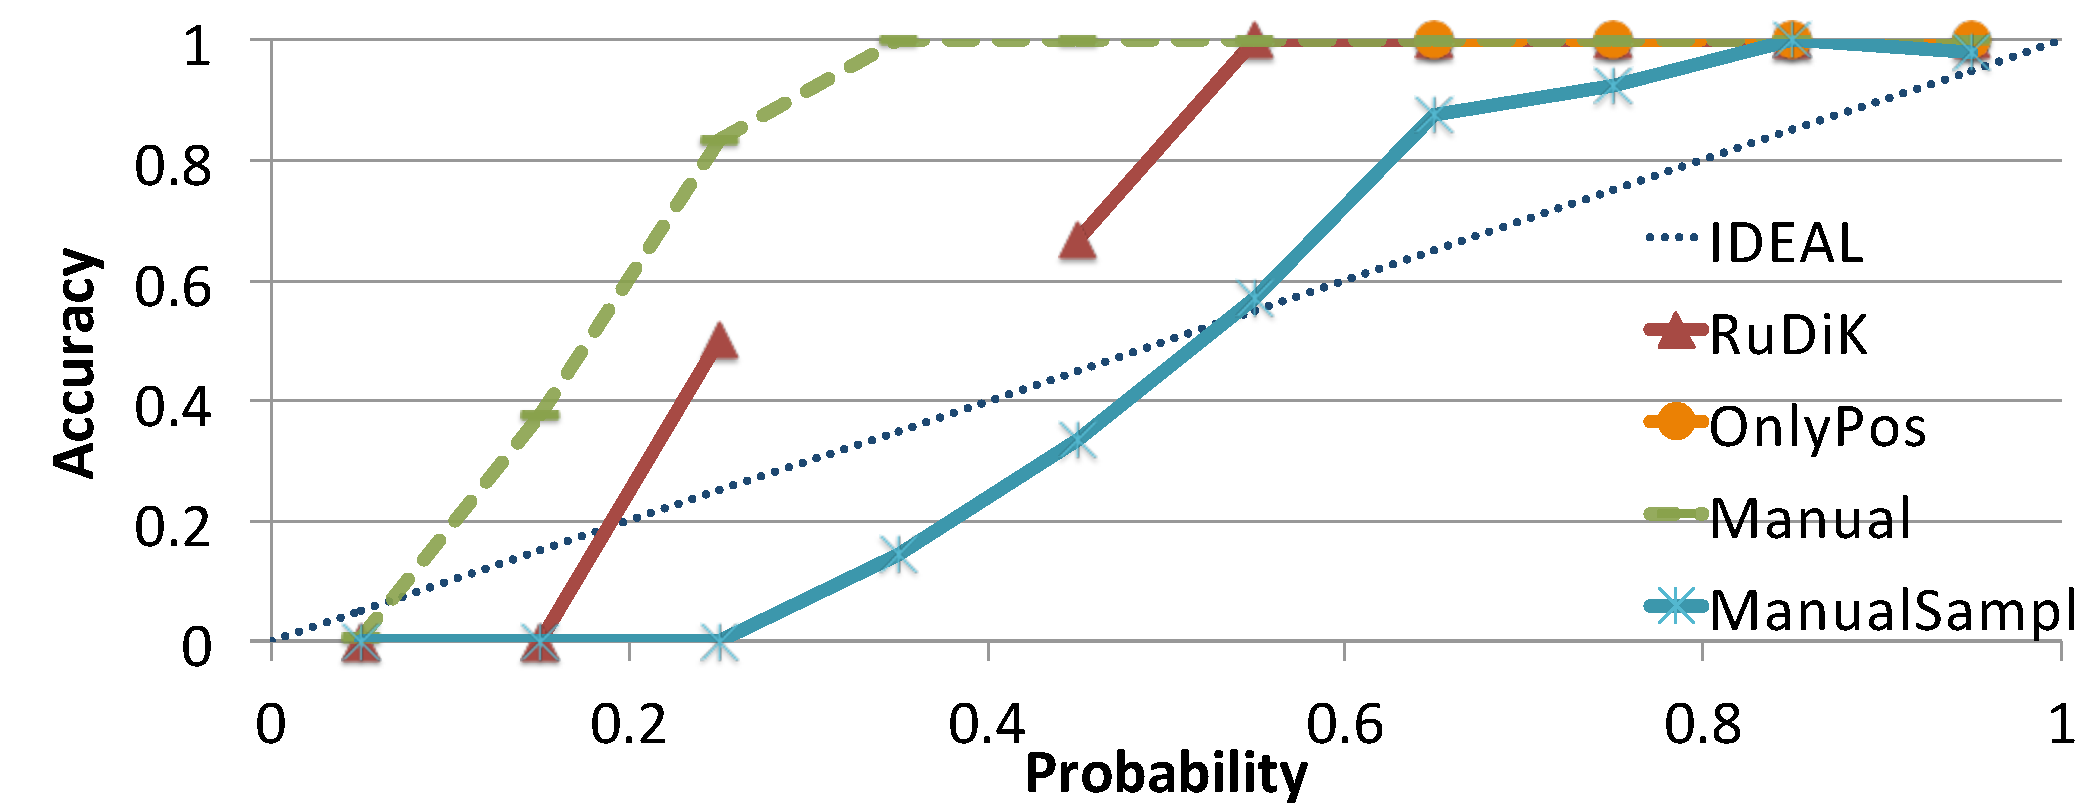
\includegraphics[width=.95\columnwidth]{include/figure/deepDive1K.pdf}
	\vspace{-1ex}
	\caption{\deepdive executions with different training examples -- 1K articles.}
	\label{fig:deep_dive_1k}
\end{figure}

%\footnote{\url{http://deepdive.stanford.edu/}}, where the goal is to extract mentions of married people from text articles
 %We used \deepdive spouse showcase example. \deepdive already provides some negative rules to generate negative examples (e.g., if two people appear in a sentence connected by the words \textit{brother} or \textit{sister} then they are not married). We therefore compare the output of \deepdive using our generated negative examples and the ones generated with \deepdive rules. 
%
Figure~\ref{fig:deep_dive_1k} shows \deepdive accuracy plot run on 1K input documents. The accuracy plot shows the fraction of correct positive predictions over total predictions (y-axis), for each output probability value (x-axis). The perfect algorithm, marked by the dotted blue line, would predict all facts with a probability of 1 and zero facts with an output probability of 0.
% which is the idealistic expected behavior marked by the dotted blue line. 
The best algorithm deflects the least from the blue dotted line, and this is our evaluation metric.
%The dotted blue line represents the ideal situation, where the system finds high number of evidence positive predictions for higher probability output values -- when the output probability is 0 there should not be positive predictions. 
%The plot is computed over a test set, while the system is trained over a separated training set. 
Figure shows 4 lines other than the ideal one. \krd is the output of \deepdive using our approach to generate negative examples. \texttt{OnlyPos} uses only positive examples from \dbpedia, \texttt{Manual} uses positive examples from \dbpedia and manually defined rules to generate negative examples, while \texttt{ManualSampl} uses only a sample of the manually generated negative examples in size equal to positive examples. \texttt{OnlyPos} and \texttt{Manual} do not provide valid training, as the former has only positive examples and labels everything as true, while the latter has many more negative examples than positive and labels everything as false. \texttt{ManualSampl} is the clear winner, while our approach suffers from the absence of data: over the input 1K articles, we found only 20 positive and 15 negative examples from \dbpedia.
The lack of evidence in the training data also explains the missing points for \krd in the chart, where there were no predictions in the probability range 25-45\%.

\begin{figure}[ht]
	\centering
	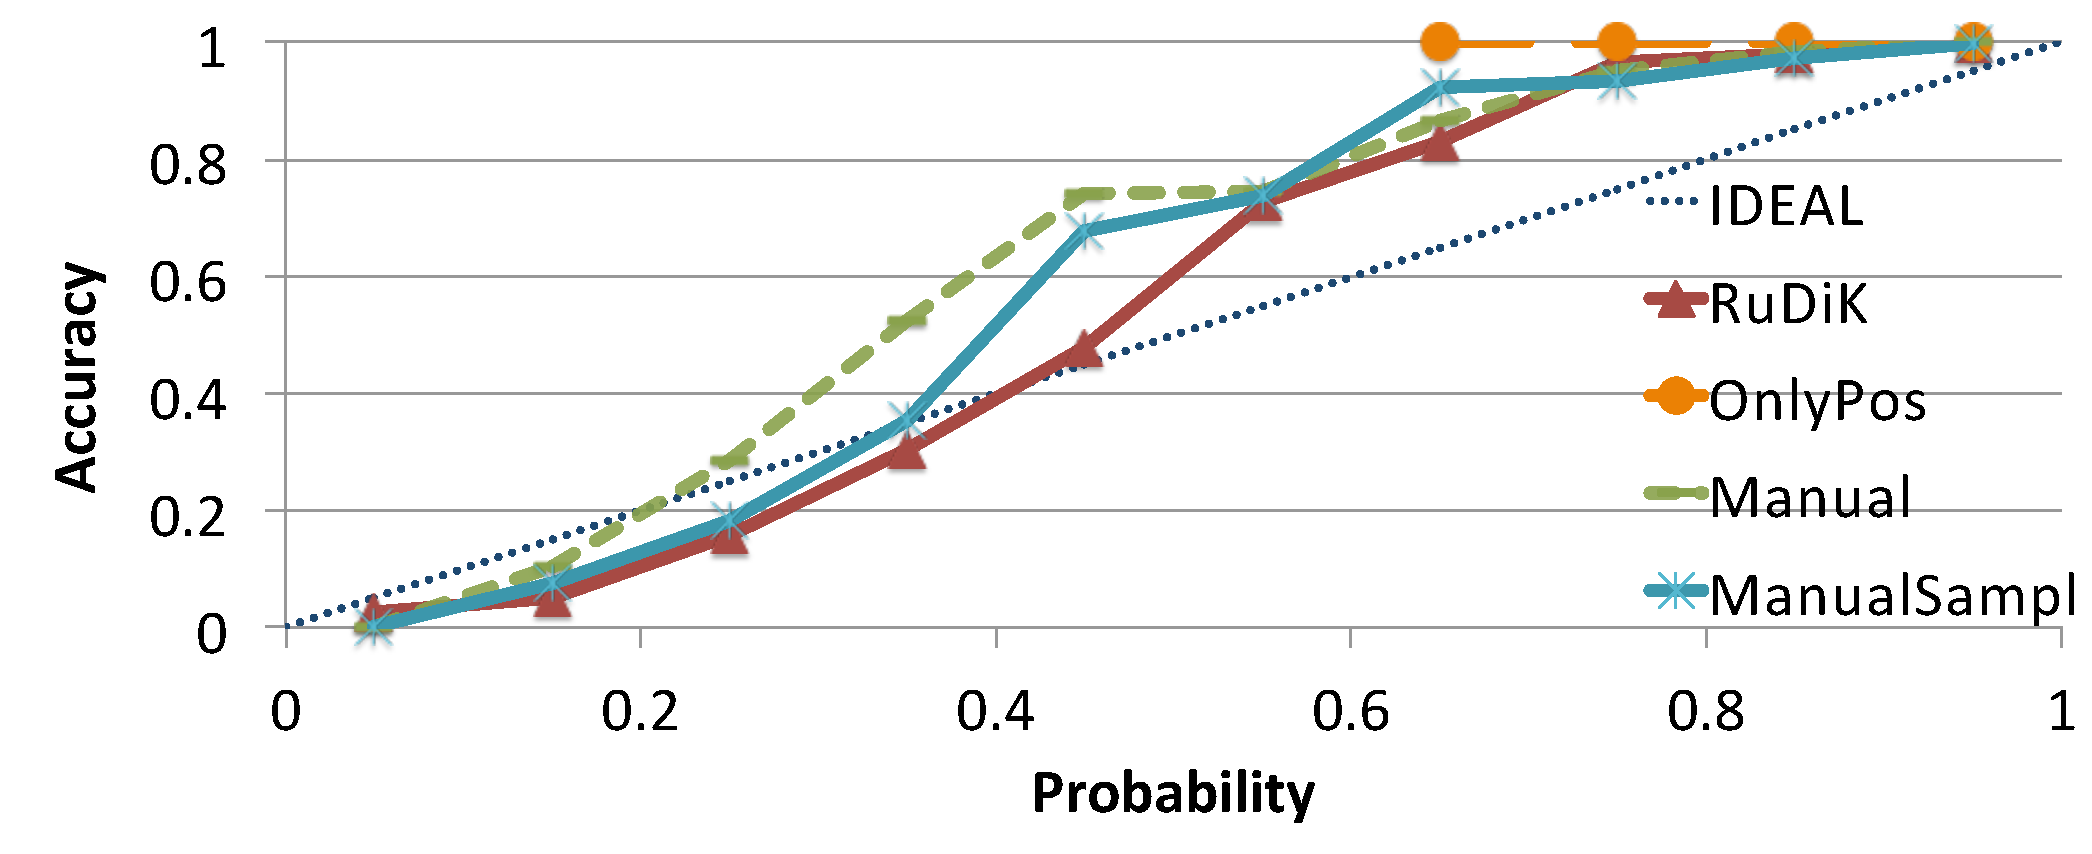
\includegraphics[width=.95\columnwidth]{include/figure/deepDive1M.pdf}
		\vspace{-1ex}
	\caption{\deepdive executions with different training examples -- 1M articles.}
	\label{fig:deep_dive_1M}
\end{figure}

When we extend the input to 1M articles, things change drastically (Figure~\ref{fig:deep_dive_1M}). All approaches except \texttt{OnlyPos} can successfully drive \deepdive in the training, with the examples provided with \krd leading to a slightly better result. This is because of the quality of the negative examples: our rules generate representative examples that help \deepdive in understanding discriminatory features between positive and negative labels.
The output of \texttt{ManualSampl} and \krd are very similar, meaning that we can use our approach to simulate user behaviour and automatically produce negative examples. 
%NOT ESSENTIAL
%With manually defined rules the number of generated examples is significantly higher ($23$K vs $5$K generated with \krd), however the results are very similar since a small number of significant examples is enough to provide complete evidence for the training. 
%This confirms the main finding of this experiment: as long as we have an external source of information with a decent coverage over the input articles, users do not need to worry about providing rules to generate negative examples.

\vspace{-1ex}
\subsection{Internal Evaluation} \label{sec:krd_int_evaluation}
We briefly outline some of the most relevant findings when studying the impact of individual components in \krd.
Full results on the internal evaluation %are not reported due to space reasons but 
can be found in the technical report online at \url{http://bit.ly/2bDZO9F}.

\begin{table}[htb]
	\centering
	\caption{Effect of Negative Examples Generation Strategy on \dbpedia.}
	\label{tab:random_neg_examples}
	\begin{tabular}{|c|c|c|c|c|}
		\hline
		\hline
		{\it Strategy}&{\it \# Potential Errors} & {\it Precision} \tabularnewline
		\hline
		\emph{Random} & 247 & \textbf{95.95}\%\tabularnewline
		\emph{LCWA\_Random} & 263 & 95.82\% \tabularnewline
		\krd & \textbf{499} & 92.38\%\tabularnewline
		\hline
	\end{tabular}
\end{table}


\noindent \myparagraph{LCWA} We demonstrate the validity of our LCWA-based generation of negative examples, which clearly outperforms random generation strategies in terms of accuracy.
Table~\ref{tab:random_neg_examples} reports the accuracy of discovering negative rules with the three different generation strategies: \krd generation strategy, random (randomly select $k$ pairs $(x,y)$ from the Cartesian product s.t. triple $\<x,p,y\> \notin \kb$), LCWA (\krd generation strategy without the constraint that $x$ and $y$ must be connected by a predicate different from $p$).
\emph{Random} and \emph{LCWA\_Random} strategies show very similar behaviours, with a slightly better precision than \krd. This is because whenever we randomly pick examples from the Cartesian product of subject and object, the likelihood of picking entities from a different time period is very high, and negative rules pivoting on time constraints are usually correct. Instead, the constriction of forcing $x$ and $y$ to be connected by a different predicate generates  negative examples with heterogeneous properties that lead to different results. Rules such as $\atom{parent}{a}{b} \Rightarrow \neg \atom{spouse}{a}{b}$ are very unlikely to be generated with random strategies, since the likelihood of picking two people that are in a parent relation is very low. The generation strategy we adopt in \krd allows the discovery of more types of rules, and not only rules involving time constraints. 


\noindent \myparagraph{Literals} Including literals in the mining is especially beneficial for negative rules, where we double the number of errors discovered with a 10\% increase in precision.

\noindent \myparagraph{Path Length} $maxPathLen=3$ is the optimal value for the length parameter: with smaller values we lose several meaningful rules, and with bigger values we do not gain in precision while increasing the election time by an order of magnitude. % or errors detected.

\noindent \myparagraph{Weight Parameters} An empirically validation supports the choice of the values used for $\alpha$ and $\beta$ in both positive and negative settings. As expected, high $\alpha$ leads to higher recall with lower precision. In both positive and negative settings, the variation in performance for $\alpha \in [0.1,0.9]$ is anyway limited ($\leq 12\%$), showing the robustness of the set cover problem formulation.

\noindent \myparagraph{Search} The $A^*$ search algorithm and pruning reduces by more than 50\% the average running time with peaks of an order of magnitude compared to a baseline algorithm that generates the universe of all possible rules and applies the greedy set cover algorithm on it.

\noindent \myparagraph{Set Cover} Our set cover problem formulation leads to better rules in the output w.r.t. a ranking based solution. Correct rules oftentimes are not among the top-10 ranked, and we found cases where meaningful rules are below the 100$^{th}$ position.
	
	%there exist good rules ranked as low as the hundreds (e.g., a good rule 120$^{th}$ in the ranking). 
	%stefano please check this number <<<<
	%This emphasize upon the fragility in ranking mechanisms.

%CANNOT AFFORD TO INCLUDE ALL INTERNATAL EVALUATION
%In this last set of experiments we measured the impact of \krd relevant features in order to quantify the benefit of three main aspects in rule discovery. 
%We run \krd on \dbpedia with different settings than the standard ones.
%We report results on the same top-5 predicates of Section~\ref{sec:gen_evaluation} for both positive and negative rules.
%
%\myparagraph{Effect of Literals}
%Since previous KB rule discovery approaches exclude literals from the mining~\cite{abedjan2014amending,galarraga2015fast} (TODO: cite Sigmod ontological), we wanted to quantify the impact of having literal rules. Thus we run \krd excluding all literal values. Table~\ref{tab:literals_effect} reports the output precision with and without literals.
%\begin{table}[b]
%	\centering
%	
%	\begin{small}
%		\begin{tabular}{c|c|c|c|c|}
%			\cline{2-5}
%			& \multicolumn{2}{c|}{\textbf{With Literals}} & \multicolumn{2}{c|}{\textbf{Without Literals}} \tabularnewline
%			\hline
%			\multicolumn{1}{ |c| }{\it Type}&{\it Run Time} & {\it Precision} &{\it Run Time} & {\it Precision} \tabularnewline
%			\hline
%			\multicolumn{1}{ |c| }{Positive Rules} & $\sim$35min & \textbf{63.99}\% & $\sim$54min & 60.49\%\tabularnewline
%			\multicolumn{1}{ |c| }{Negative Rules} &  $\sim$20min & \textbf{92.38}\% (499) &$\sim$25min &84.85\% (235) \tabularnewline
%			\hline
%		\end{tabular}
%	\end{small}
%	\caption{Rules Accuracy without Literals on \dbpedia.}
%	\label{tab:literals_effect}
%\end{table}
%Including literal values in the mining has a considerable impact on final accuracy, both for positive and negative rules. The effect is particularly evident for negative rules, where excluding literals involves finding less than half potential errors (numbers in brackets) with a lower precision. \texttt{founder} is the most evident example: \krd discovers 79 potential errors with a 95\% precision with literal rules, while there are not output errors with rules without literals.
%
%Surpisingly, including literals reduces also the running time. This is due to the pruning effect of the $A^*$ search: if we include literals the algorithm can find rather soon valid literal rules, which causes the pruning of several paths on the graph. If we exulted literals instead these paths cannot be pruned and needs to be inspected by the algorithm, which entails a bigger search space.
%
%\myparagraph{Rules Length Impact}
%The $maxPathLen$ parameter fixes the maximum number of atoms allowed in the body of a rule. Low values for $maxPathLen$ may exclude from the search space meaningful rules, while high values may exponentially increase the search space and consequently the running time. Table~\ref{tab:rules_len_impact} reports
%\begin{table}[htt]
%	\centering
%	\caption{$maxPathLen$ Parameter Impact on \dbpedia.}
%	\label{tab:rules_len_impact}
%	\begin{small}
%		\begin{tabular}{c|c|c|c|c|c|c|}
%			\cline{2-7}
%			& \multicolumn{2}{c|}{$MaxPathLen$ = \textbf{2}} & \multicolumn{2}{c|}{$MaxPathLen$ = \textbf{3}} & \multicolumn{2}{c|}{$MaxPathLen$ = \textbf{4}}\tabularnewline
%			\hline
%			\multicolumn{1}{ |c| }{\it Type}&{\it Run Time} & {\it Precision} &{\it Run Time} & {\it Precision} &{\it Run Time} & {\it Precision} \tabularnewline
%			\hline
%			\multicolumn{1}{ |c| }{Positive} & \textbf{$\sim$3min}& 49.17\% & $\sim$35min & \textbf{63.99}\% & & \tabularnewline
%			\multicolumn{1}{ |c| }{Negative} & \textbf{$\sim$56sec} & 90\% (131) & $\sim$20min & \textbf{92.38}\% (499)& & \tabularnewline
%			\hline
%		\end{tabular}
%	\end{small}
%\end{table}
%accuracy values and run times for different $maxPathLen$ settings. If we set $maxPathLen=2$ we observe a significant improvement in running time, at the expense of loosing several meaningful rules. In particular we loose all the rules that involve literals comparison, as these require a minimum of three atoms in the body. This is particularly evident for negative rules, where we spot a fewer number of errors (in round brackets) with a lower precision. At the other side of the spectrum, with $maxPathLen=4$ the search space explodes and \krd was not capable of finishing the computation within 24 hours for each predicate. We therefore report the accuracy of rules discovered in 24 hours of computation. The results are comparable to those computed with $maxPathLen=3$, provided the absence of rules that might have been discovered after 24 hours. Furthermore, we did not notice any new discovered correct rule with body length equal to 4. Rules with length 4 are usually very complex to understand, and when executed over the KB they often return an empty result (i.e., they are useless both for discovering additional information and for identifying inconsistencies). Here a couple of examples of output rules with length 4:
%
%%NOT ESSENTIAL
%%\vspace{-5ex}
%%{\scriptsize
%%	\begin{gather*}
%%		\atom{birthPlace}{a}{v_0} \wedge \atom{areaTotal}{v_0}{v_1} \wedge \atom{viafId}{b}{v_2} \wedge v_1 < v_2 \Rightarrow \neg \atom{academicAdvisor}{a}{b} \\
%%		\atom{foundingYear}{a}{v_2} \wedge \atom{birthPlace}{b}{v_0} \wedge \atom{foundingYear}{v_1}{v_2}  \wedge \atom{foundationPlace}{v_1}{v_0} \Rightarrow \atom{founder}{a}{b}
%%	\end{gather*}
%%}
%%We therefore decided that $maxPathLen=3$ is a good compromise between a reasonable running time and a good output accuracy.
%
%\myparagraph{Negative Examples Generation}
%A key point in \krd is the generation of negative examples with a modified version of the LCWA (Section~\ref{sec:ex_generation}). We therefore evaluate two different strategies to generate negative examples. Given a target predicate $p$ from a KB $\kb$, we call $t_a$ the most common type of entities that are subject of $p$, and $t_b$ the most common type for the object. As an example, if $p=$\texttt{founder}, $t_a=Company$ and $t_b=Person$. We define $k$ as the number of triples having $p$ as predicate in $\kb$ -- $k$ is the cardinality of the positive examples set. The first alternative negative examples generation strategy is \emph{Random}: we randomly select $k$ pairs $(x,y)$ from the cartesian product of all entities $x$ of type $t_a$ and all entities $y$ of type $t_b$, such that the triple $\<x,p,y\> \notin \kb$. The second generation strategy, named ${LCWA}\_Random$, leverages on the LCWA. In $LCWA\_Random$ we randomly pick $k$ pairs $(x,y)$ from the cartesian product of all entities $x$ of type $t_a$ and all entities $y$ of type $t_b$, such that:
%\begin{inparaenum}[\itshape(i)]
%	\item $\<x,p,y'\> \in \kb$, with $y' \neq y$;
%	\item $\<x',p,y\> \in \kb$, with $x' \neq x$;
%	\item $\<x,p,y\> \notin \kb$.
%\end{inparaenum}
%$LCWA\_Random$ is equivalent to \krd generation strategy, minus the constriction that $x$ and $y$ must be connected by a predicate different from $p$. The constraint of having $k$ examples aims at reducing the size of the cartesian product that can easily explode otherwise.
%
%Table~\ref{tab:random_neg_examples} reports the accuracy of discovering negative rules with the three different generation strategies (\krd is our modified LCWA strategy).
%\begin{table}[t]
%	\centering
%	\caption{Effect of Negative Examples Generation Strategy on \dbpedia.}
%	\label{tab:random_neg_examples}
%	\begin{tabular}{|c|c|c|c|c|}
%		\hline
%		\hline
%		{\it Strategy}&{\it \# Potential Errors} & {\it Precision} \tabularnewline
%		\hline
%		\emph{Random} & 247 & \textbf{95.95}\%\tabularnewline
%		\emph{LCWA\_Random} & 263 & 95.82\% \tabularnewline
%		\krd & \textbf{499} & 92.38\%\tabularnewline
%		\hline
%	\end{tabular}
%\end{table}
%\emph{Random} and \emph{LCWA\_Random} strategies show very similar behaviours, with a slightly better precision than \krd. This is because whenever we randomly pick examples from the cartesian product of subject and object, the likelihood of picking entities from a different time period is very high, and negative rules pivoting on time constraints are usually correct.
%As an example, a correct rule for the target predicate \texttt{child} is $\atom{birthDate}{a}{v_0} \wedge \atom{birthDate}{b}{v_1} \wedge v_0 > v_1 \Rightarrow \neg \atom{child}{a}{b}$, stating that whenever a person $a$ is born after a person $b$, then $b$ cannot be child of $a$.
%The likelihood of randomly picking some pairs of persons $(x,y)$ where $x$ is born after $y$ is very high, hence such kind of rules will often be discovered. However these are the \emph{only} kind of rules that random generation strategies are able to find, as shown from the smaller number of errors that they can identify. 
%Instead, the constriction of forcing $x$ and $y$ to be connected by a different predicate generates  negative examples with heterogeneous properties that lead to different results. Rules such as $\atom{parent}{a}{b} \Rightarrow \neg \atom{spouse}{a}{b}$ are very unlikely to be generated with random strategies, since the likelihood of picking two people that are in a parent relation is very low. The generation strategy we adopt in \krd allows the discovery of more types of rules, and not only rules involving time constraints. This has multiple benefits: on the one hand, we discover more rules, which entails discovering a higher number of errors (Table~\ref{tab:random_neg_examples}); on the other hand, different rule types lead to high quality negative examples, that can be used in several applications such as training Machine Learning algorithms (see Section~\ref{sec:krd_deep_dive}).
%
%\myparagraph{Effect of Weight Parameters}
%\begin{figure}[t]
%	\centering
%	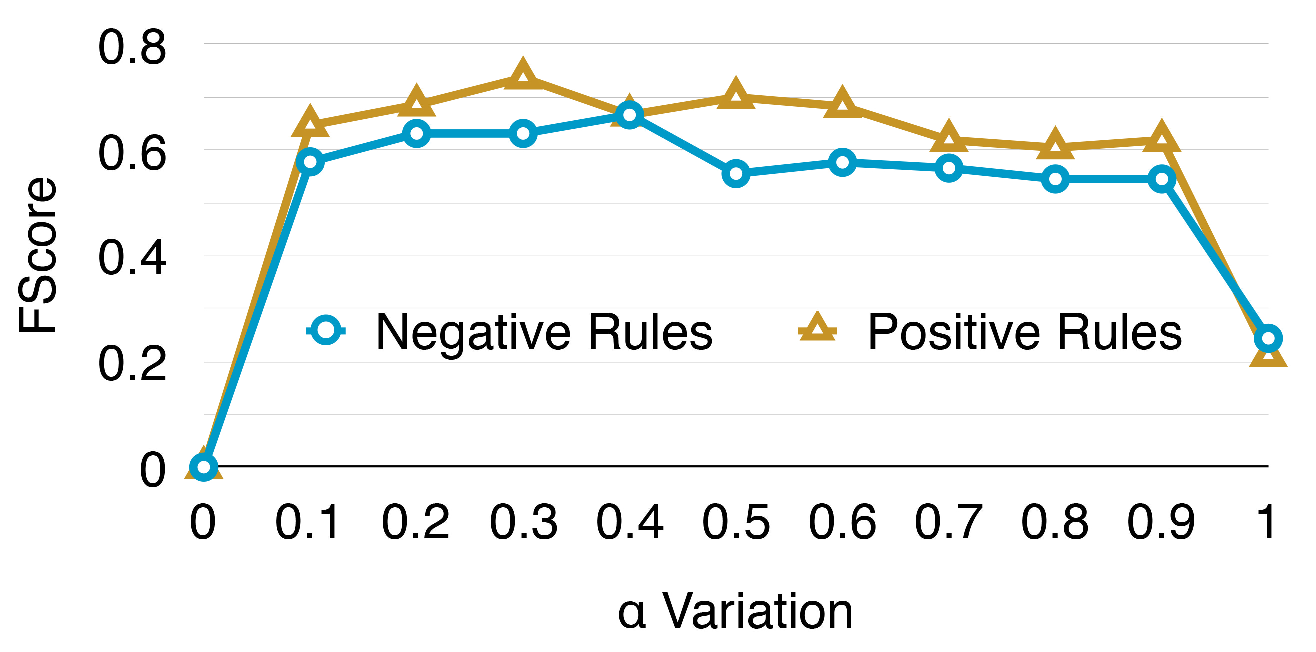
\includegraphics[width=0.9\columnwidth]{include/figure/alpha_impact.pdf}
%	\caption{$\alpha$ Parameter Performance Impact}
%	\label{fig:alpha_impact}
%\end{figure}
%Our weight function is ruled by two different parameters: $\alpha$ and $\beta$, with $\alpha \in [0,1]$ and $\beta=1-\alpha$ (Section~\ref{sec:krd_weight_fun}). This experiment aims at establishing the optimal value to assign to $\alpha$ and $\beta$, and to quantify the impact of the two parameters on the overall performance. We recall that $\alpha$ quantifies the relevance of the coverage over the generation set, while $\beta$ is the importance of the coverage over the validation set. In other words, a high $\alpha$ supports high recall over precision, while a high $\beta$ supports a high precision over recall. Figure~\ref{} shows the variation of \textsf{$F_1$-Score} with different values of $\alpha$ for both positive and negative rules on \dbpedia. For each different run, we manually label each output rule as true or false, where the total number of correct rules for each predicate is the union of all possible correct rules over all the runs. We then compute \textsf{Precision}, \textsf{Recall}, and \textsf{$F_1$-Score} at rule level. On the one hand, setting $\alpha=0$ produces an empty output, since we neglect the coverage over the generation set and we are just after rules that do not cover any element of the validation set. On the other hand, setting $\alpha=1$ means chasing rules just based on the coverage over the generation set, no matter what the coverage over the validation set is. This strategy ends up in producing a huge amount of rules (high recall), with very few correct rules (low precision). Correct values lie somewhere in between. For positive rules, the best assignment is $\alpha=0.3$ and $\beta=0.7$. Since discovering correct positive rules is more challenging than negative ones, favoring precision over recall gives the best accuracy. For negative rules instead, the best assignment is $\alpha=0.4$ and $\beta=0.6$. Since negative rules are often correct, we can relax the constraint over precision and be slightly more recall oriented. In both cases, the variation in performance for $\alpha \in [0.1,0.9]$ is anyway limited ($\leq 12\%$), showing the robustness of the set cover problem formulation.
%
%\myparagraph{$A^*$ pruning impact}
%\begin{figure}[b]
%	\centering
%	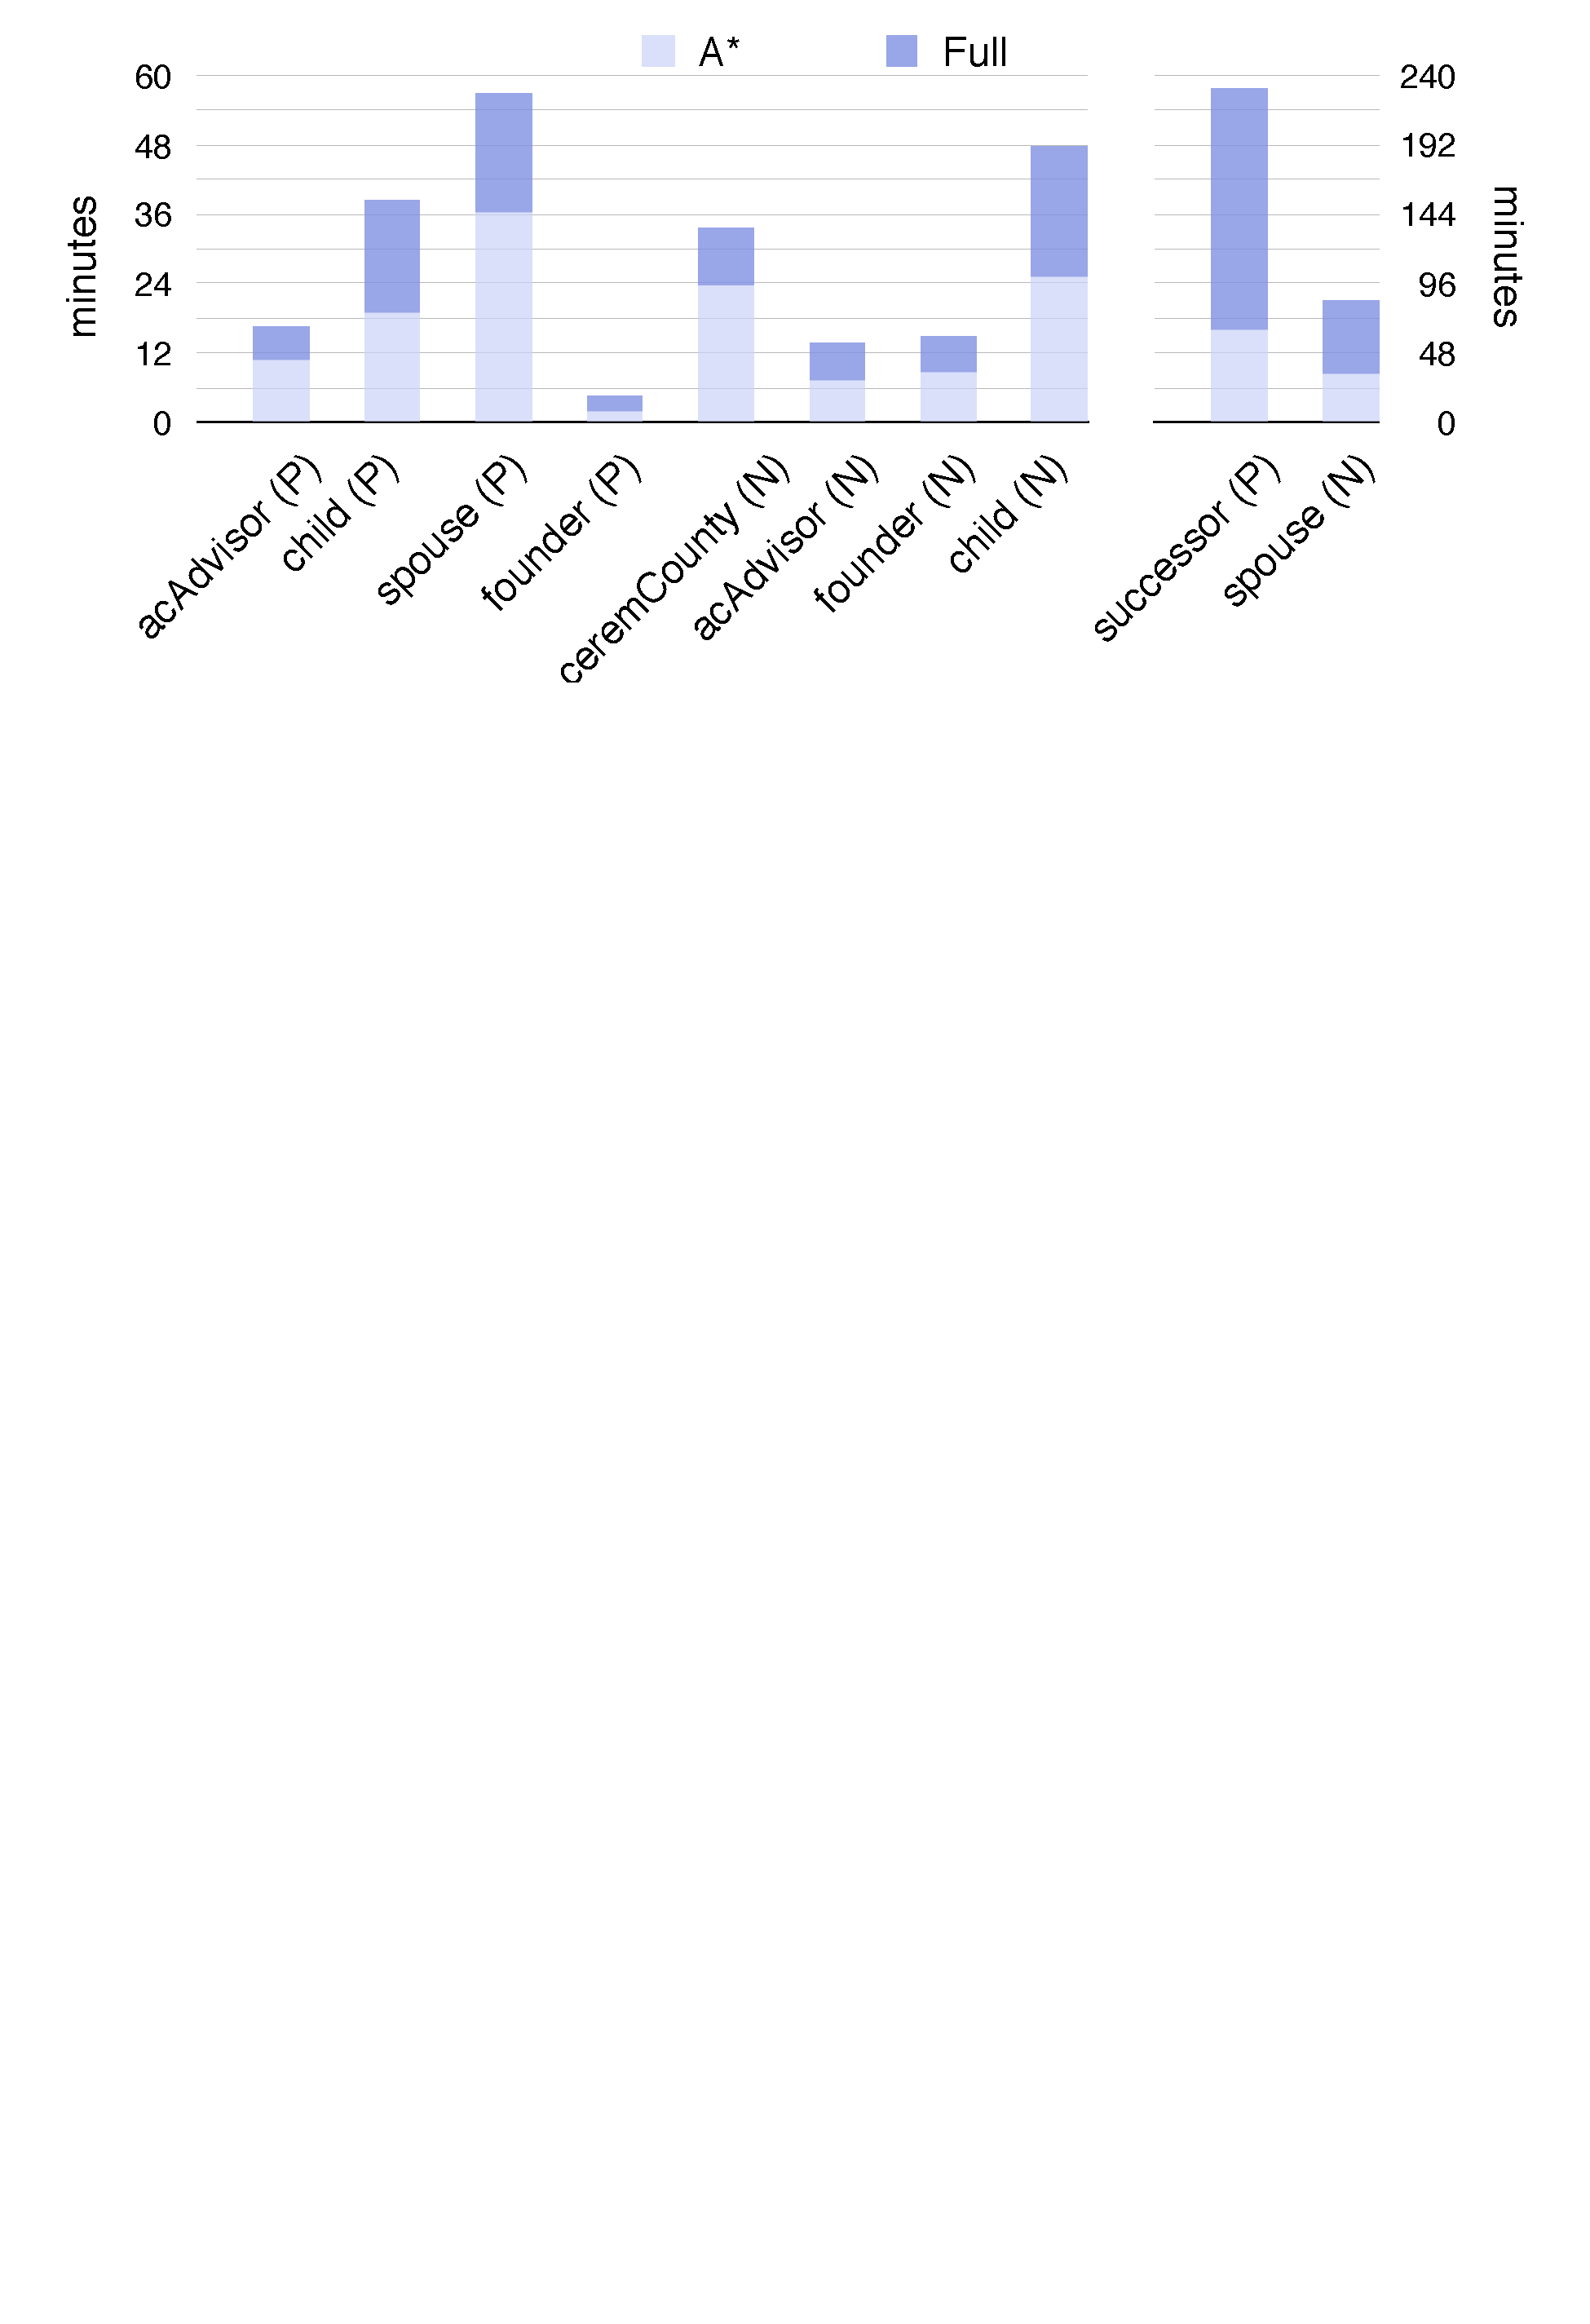
\includegraphics[width=\columnwidth]{include/figure/a*_runtime_improv.pdf}
%	\caption{$A^*$ Pruning Runtime Improvement}
%	\label{fig:pruning_impact}
%\end{figure}
%Another aspect we wanted to quantify is the benefit brought by the $A^*$ algorithm on the overall running time. Figure~\ref{fig:pruning_impact} shows the running time, for each target predicate, of the $A^*$ algorithm (light-colored bars) against a modified version that first generates the universe of all possible rules, and then apply the greedy set cover algorithm on such a universe (dark-colored bars). For the last two predicates refer to the y-axis labels on the right hand side, as these predicates have a significant higher running time. In the figure \texttt{(P)} refers to positive rules, while \texttt{(N)} to negative rules.
%The $A^*$ strategy allows the pruning of several unpromising paths and avoids the generations of such paths from the disk. This is directly reflected on running times, where we notice an average 50\% improvement. When there exist rules that cover many examples from the generation set (e.g., \texttt{successor (P)}, \texttt{founder (P)}), the algorithm is capable of identifying such rules rather early, thus pruning several unpromising paths that cover a subset examples from the generation set. In such cases the running time improvement is above 70\%.
